\lstdefinestyle{mycode}{
  belowcaptionskip=1\baselineskip,
  breaklines=true,
  xleftmargin=\parindent,
  showstringspaces=false,
  basicstyle=\footnotesize\ttfamily,
  keywordstyle=\bfseries,
  commentstyle=\itshape\color{gray!40!black},
  stringstyle=\color{ao},
  numbers=left,
  numbersep=5pt,
  numberstyle=\tiny\color{gray},
}
\lstset{escapechar=@,style=mycode}


\title{Специализация машинного кода}

\titlerunning{Специализация машинного кода}

\author{Кравченко Юрий}

\authorrunning{Кравченко Юрий}

\tocauthor{Кравченко Юрий}
\institute{СПбАУ\\
	\email{krav4enkoyura@yandex.ru}}

\maketitle

\begin{abstract}
Данная работа посвящена исcледованию возможности реализации самоприменимого специализатора для
машинного кода.
В работе выявлены ключевые особенности специализации, возникающие в контексте специализации машинного
кода, предложены методы решения некоторых конкретных задач.
Также в работе представлен базовый алгоритм специализации машинного кода и
описана реализация прототипа специализатора машинного кода на языке \textsf{C},
проведена аппробация его возможностей.
\end{abstract}


%#################
\section*{Введение}
В современном мире оптимизация программ является неотъемлемой частью процесса разработки программного обеспечения. Существует огромный спектр методов оптимизации.
Одни делают оптимизации на уровне языка, другие оптимизируют уже скомпилированную программу или одно из её возможных промежуточных
представлений.
Часть предназначена для оптимизации вызовов функций, другие же специализируются на работе с многопоточными приложениями.
На фоне данного многообразия, выделяется подход, называемый \emph{специализацией}.
Программный компонент, производящий специализацию, называется \emph{специализатором} (specializer) или
\emph{частичным вычислителем} (partial evaluator).
Специализатор $spec$ принимает на вход программу $p$ (её исходный код) и часть её входных данных $in_1$.
Результатом работы специализатора является программа $p_{spec}$.
Она представляет из себя оптимизированную версию программы $p$, согласованную с известной частью входных данных $in_1$.
Программа $p_{spec}$ принимает на вход оставшуюся часть входных данных программы $p$ и выдаёт такой же результат,
что и программа $p$ на всех входных данных. 
$$\begin{array}{l l c l}
    \llbracket spec \rrbracket_{L_2} & [p, in_1] &= &p_{spec}\\
    \llbracket p_{spec} \rrbracket_{L_1} & [in_2 ,\dots] &= &out
  \end{array}$$
      
Выполнение данного свойства и является определением специализатора. Важной отличительной чертой специализации, является то, что для применения метода необходимо знать часть входных данных программы. Это позволяет гораздо эффективнее оптимизировать программы, но сужает сферу применения этого метода.

В 1973 году Футамура (Y. Futamura) предложил использовать специализацию для несколько других целей и сформулировал проекции Футамуры--Ершова--Турчина~\cite{Futa}. Идея проекций заключается в следующем. Положим, нам даны язык $L$, самоприменимый специализатор для языка $L$ и интерпретатор некоторого языка $R$ на языке $L$. Самоприменимость специализатора значит, что он может принимать себя в качестве входных данных. В частности, из этого следует, что язык реализации интерпретатора должен совпадать с языком, который он может принимать на вход. Первая проекция говорит о том, что при специализации интерпретатора на программу на языке $R$ получится семантически эквивалентная программа, но на языке $L$. Вторая проекция говорит о том, что при самоприменении специализатора на интерпретатор получится компилятор из языка $R$ в язык $L$. Третья проекция говорит о том, что при самоприменении специализатора на себя же, получается генератор компиляторов $compGen$, который принимает на вход интерпретатор и возвращает компилятор.
    $$
    \begin{array}{l l l c l}
      I & \llbracket spec \rrbracket_L &[int, p] &= &q\\
      II & \llbracket spec \rrbracket_L &[spec, int] &= &comp\\
      III & \llbracket spec \rrbracket_L &[spec, spec] &= &compGen
    \end{array}$$  

Таким образом, специализация программ может быть использована для автоматического преобразования
интерпретатора языка программирования в его компилятор.
Одной из особенностей генерируемых таким образом компиляторов является то, что их целевым языком
всегда является целевой язык специализатора, он же --- язык реализации интерепретатора.
Ввиду того, что реализация специализаторов для языков программирования является чрезвычайно трудоёмкой
задачей, а иногда и неразрешимой, существующие специализаторы имеют своим целевым языком либо
некотороый академический язык программирования, либо весьма ограниченный прототип одного из существуюших
высокоуровневых языков.
Реалазация самоприменимого специализатора для низкоуровнего представления или для машинного кода
позволила бы преобразовать произвольный интерпретатор, написанный на любом компилируемом языке, в
классический компилятор.
На данный момент не существует самоприменимых специализаторов машинного кода,
более того, эта область специализации является весьма малоисследованной.
Данная работа посвящена именно иследованию возможности реализации самоприменимого специализатора для
машинного кода.
В работе выявлены ключевые особенности специализации, возникающие в контексте специализации машинного
кода, предложены методы решения некоторых конкретных задач.
Также в работе представлен базовый алгоритм специализации машинного кода и
описана реализация прототипа специализатора машинного кода на языке \textsf{C},
проведена аппробация его возможностей.
Предложенный прототип специализатора не обладает возможностью к самоприменению,
но является первым, реализующим первую проекцию Футамуры для машинного кода.
Данная работа может являться отправной точкой для дальнейших исследований в области самоприменимых
специализаторов машинного кода.


\section{ Введение в область}
В этой главе рассмотрены некоторые понятия, необходимые для дальнейшего понимания данной работы.

\subsection{ Машинный код}
Машинный код~\cite{AMD} представляет собой набор инструкций, которые способны исполняться непосредственно на процессоре. Программа в машинном коде представляет собой список команд, представленный в виде двоичного кода. В дальнейшем под машинным кодом будет подразумеваться машинный код для архитектуры x86-64.

\subsection{ Проекции Футамуры~\cite{Futa}}
Пусть $spec$ --- специализатор языка $S$, написанный на языке $S$, $int$ --- интерпретатор языка $L$ на языке $S$, $p$ --- программа на языке $L$, а $in$ --- входные данные для этой программы. Специализатор $spec$ может принимать в качестве входных данных любую программу на языке $S$ и часть её входных данных. Интерпретатор $int$ является программой на языке $S$ и может принимать в качестве входных данных любую программу на языке $L$ и её входные данные. Значит, специализатор $spec$ может принять в качестве входных данных интерпретатор $int$ и программу $p$. Рассмотрим, что получится в результате такого применения. По определению специализатора, получается некая программа $q$ на языке $S$ такая, что если ей передать в качестве входных данных некий $in$, результат будет равен результату исполнения интерпретатора $int$ на программе $p$ и входных данных $in$, что в свою очередь по определению интерпретатора равно результату исполнения программы $p$ на входных данных $in$. То есть при вызове программ $p$ и $q$ на одних и тех же входных данных, получается один и тот же результат. Ключевая разница между программами $p$ и $q$ состоит в том, что они написаны на разных языках: $p$ на языке $L$, а $q$ --- на языке $S$. Это значит, что данное применение специализатора позволяет скомпилировать программу из языка, для которого написан интерпретатор, в язык реализации интерпретатора. Данный результат называется первой проекцией Футамуры.
$$\llbracket spec \rrbracket_L [int, p] = q$$

Специализатор $spec$, как и интерпретатор $int$, является программой на языке $S$ и входные данные для него тоже состоят из двух частей. Значит его можно специализировать. Передадим специализатору $spec$ в качестве входных данных самого себя и интерпретатор $int$. По определению специализатора, получается некая программа $comp$ на языке $S$ такая, что если ей передать в качестве входных данных программу $p$, результат будет равен результату первой проекции Футамуры, то есть программе $q$. Таким образом, программа $comp$ является компилятором, способным переводить программы с языка $L$ на язык $S$. Данный результат называется второй проекцией Футамуры.
$$\llbracket spec \rrbracket_L [spec, int] = comp$$

Продолжая этот ряд, передадим специализатору $spec$ в качестве входных данных самого себя дважды. По определению специализатора, получается некая программа $compGen$ на языке $S$ такая, что если ей передать в качестве входных данных интерпретатор $int$, результат будет равен результату второй проекции Футамуры, то есть программе $comp$.
Таким образом, программа $compGen$ является генератором компиляторов, так как способна по интерпретатору языка генерировать его компилятор.
Данный результат называется третьей проекцией Футамуры. 
$$\llbracket spec \rrbracket_L [spec, spec] = compGen$$


\section{Существующие подходы к специализации низкоуровневых языков программирования}

Как уже отмечалось ранее, область специализации низкоуровневых языков программирования является малоизученной.
Это отражается в том, что существует немного исследований, посвящённых этой теме.
В этом разделе описана пара наиболее релевантных работ.
Первая посвящена специализации языка \textsf{FlowChart}, являющегося своеобразным смешением низкоуровнего
представления и \textsf{Pascal}-подобного языка~\cite{PEAPG}.
Вторая --- единственная, на сколько это известно автору, и при том недавняя,
работа по специализации машинного кода~\cite{PEMC}.

\subsection{Специализация \textsf{FlowChart}}

\begin{figure}[t]
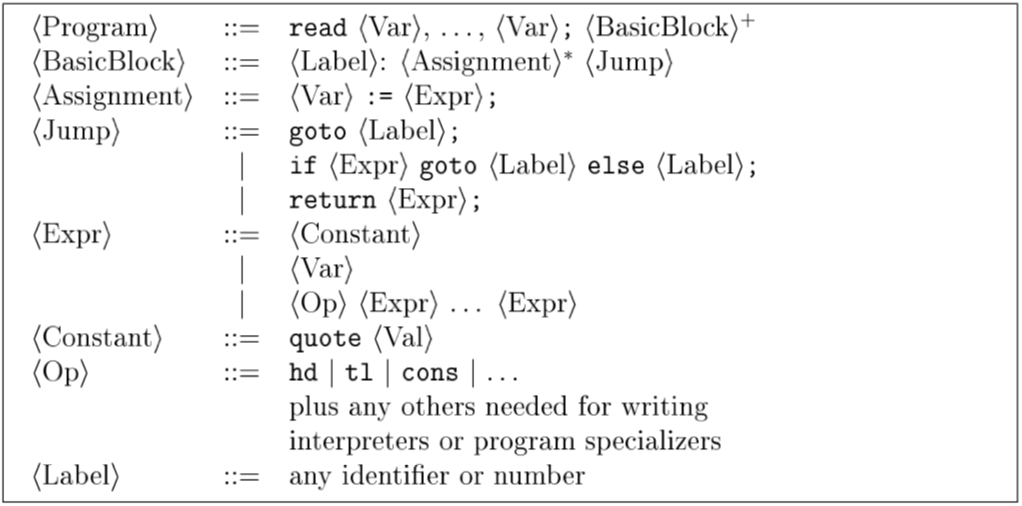
\includegraphics[width=\linewidth]{Kravchenko/Pic1.png}
\caption{Flow Chart\protect\footnotemark}
\label{fig:flow}
\end{figure}

\footnotetext{Рисунок заимствован из книги~\cite{PEAPG}, страница 70.}

В  книге~\cite{PEAPG} помимо прочего идёт речь о специализации языка \textsf{FlowChart}. Синтаксис этого языка представлен на рисунке~\ref{fig:flow}.

Можно заметить что данный язык напоминает машинный код своей структурой: программа представляет собой блоки, переход между которыми
осуществляется с помощью условных и безусловных переходов.
Также, алгоритм, предложенный для специализации \textsf{FlowChart}, является самоприменимым.
Поэтому основные идеи, предложенные впервые при публикации этого алгоритма, были частично использованы автором при создании
алгоритма специализации машинного кода.
Алгоритм специализации языка \textsf{FlowChart} является \emph{offline} алгоритмом \emph{с постоянным разбиением} (uniform division).
Это значит, что переменные классифицируются как \emph{статические}, т.е. значения которых известны на момент времени исполнения
специализатора, или \emph{динамические}, т.е. значения которых известны только на момент времени исполнения специализированной программы,
и данная классификация не меняется в процессе специализации.
Поэтому начальный этап алгоритма представляет собой запуск отдельной фазы \emph{анализа времени связывания} (BTA) с целью постороения
\emph{разбиения} (divison) программы, т.е. проведения вышеописанной классификуации.
После этого пара из начальной программной точки: первого блока и начальных значений всех статических переменных ---
кладётся в очередь на обработку.
На следующем этапе происходит обработка очереди. Из неё извлекается первая пара и, если такая пара ещё не обрабатывалась, происходит её обработка. Обработка заключается в том, что сначала специализатор обрабатывает инструкции из тела блока, а затем --- инструкцию перехода. Инструкции тела блока обрабатываются нижеследующим образом. В случае если переменная, куда происходит запись результата инструкции, является динамической, данная инструкция упрощается и генерируется в ответ. Если же переменная является статической, то происходит вычисление правой части присваивания и результат вычисления записывается в соответствующую переменную. Специализация инструкции перехода зависит от её типа. В случае инструкции $return$, специализатор генерирует её в ответ и завершает обработку данного блока. Если инструкцией перехода является $goto$, специализатор делает переход на блок, на который указывает инструкция $goto$ и продолжает специализацию.
Если же в качестве инструкции перехода появляется $if$, специализация зависит от классификации условия этой
инструкции\footnote{Выражения, пободно переменным, классифицируются как \emph{статические}, если все переменные, входящие в него,
  являются статическими согласно построенному разбиению, или \emph{динамические} --- в противном случае.}.
В случае, если условие перехода является статическим, специализация происходит аналогично инструкции $goto$.
В случае же динамического условия, специализатор генерирует на выход данную инструкцию $if$,
после чего в очередь добавляется пара элементов: пары из обоих вариантов условных переходов и текущего значения статических переменных.
После этого специализация текущего блока заканчивается. Специализация программы заканчивается, когда заканчиваются пары в очереди. 

\subsection{Специализация машинного кода}
В статье~\cite{PEMC} речь идёт о создании специализатора машинного кода. Данный результат предлагается получить с помощью следующего алгоритма. Первым этапом является расщепление комплексных инструкций (которое более подробно разобрано в разделе~\ref{part:4.2}) на базовые. Следующий этап представляет собой BTA, во время которого инструкции программы классифицируются на статические, динамические и lifted инструкции. Lifted инструкции --- статические инструкции, результат исполнения которых используется в динамических инструкциях. Важной особенностью является то, что классифицируются именно инструкции, а не регистры или память. На следующем этапе, по аналогии с предыдущим алгоритмом, из очереди достаётся блок инструкций и состояние программы. Инструкции в блоке обрабатываются по очереди. Статические инструкции вычисляются и изменяют состояние программы. Динамические инструкции без изменений генерируются в ответ. Lifted инструкции упрощаются, после чего тоже генерируются в ответ. Упрощение lifted инструкций происходит следующим образом. Сначала они конвертируются в QFBV~\cite{QFBV} формулу, где происходит упрощение данной инструкции, после чего она конвертируется обратно. Стоит отметить, что использованная библиотека для работы с QFBV формулами является закрытой. Пополнение очереди происходи за счёт динамических условных переходов, как и в предыдущем алгоритме.

В итоге, данный алгоритм не сильно отличается от предыдущего, хоть и имеет свои особенности. Использование QFBV формул является приемлемым для специализации программ с целью оптимизации, но при самоприменении специализатора эта техника сильно усложняет специализатор, что мешает его самоприменению. Несмотря на это, в данной статье были выявлены основные проблемы специализации машинного кода и предложены их решения, которые частично были использованы в данной работе. 

\section{Особенности специализации машинного кода}

Специализация машинного кода отличается от специализации императивных или функциональных языков программирования.
В данной главе описываются проблемы и особенности, возникающие при специализации машинного кода, и методы их решения.

\subsection{Частое использование регистров}
\label{part:4.1}

\begin{wrapfigure}{R}{0.4\textwidth}
\begin{lstlisting}[xleftmargin = 20pt]
mov %esi %eax
mov 4 %eax
\end{lstlisting}
\caption{Фрагмент кода: частое использование регистров}
\label{fig:reg}
\end{wrapfigure}

При offline специализации с постоянным разбиением императивных программ, BTA в самом начале классифицирует все переменные
как статические или динамические.
Такая классификация загрубляет результат в случае, если в одной переменной могут оказаться как динамические, так и статические значения.
Нетрудно привести примеры, где из-за подобного загрубления большая часть программы становится динамической,
и специализация не приводит к желаемым результатам.
Тем не менее, в обычных программах зачастую используется множество переменных и значения, которые может принимать каждая из них,
логически связаны. {\color{red}--- TODO: WHAT????  я не понял смысла предыдущего предложения}
Поэтому данное загрубление либо никак не влияет на результат специализации, либо влияет незначительно.

При специализации машинного кода возникает обратная ситуация. Рассмотрим фрагмент кода на рисунке~\ref{fig:reg}. Пусть значение регистра $esi$ было динамическим. Тогда BTA классифицирует первую инструкцию как динамическую. Далее её результат записывается в регистр $eax$, из-за чего он тоже становится динамическим. В случае offline специализации с постоянным разбиением, данный регистр останется динамическим навсегда. Так, после выполнения второй инструкции значение регистра $eax$ останется динамическим, а не статическим со значением 4. Регистр $eax$ используется довольно часто. В частности, он используется для передачи возвращаемого значения из функций. Классификация его как динамический приведёт к тому, что все возвращаемые значения станут динамическими. Также, ввиду своей популярности, данный регистр имеет большой шанс, что в него положат динамическое значение. В результате получается, что в подавляющем большинстве программ данный регистр будет классифицирован как динамический,
и, как следствие, существенная часть программы станет динамической, что приведёт к недостаточной специализации.

Стоит отметить, что существуют и другие виды разбиения при offline специализации, позволяющие классифицировать
не переменные (или регистры, как в нашем примере), а их вхождения как статические или динамические.
Тем не менее, ввиду того, что при offline подходе BTA предшествует непосредственной самой фазе специализации,
а значит и результат BTA остаётся неизменным на всём её протяжении,
такое решение всё же является консервативным.
Таким образом, для решения вышеописанной проблемы, необходимо использовать другой, более сложный, метод специализации --- online специализация. Его отличие от offline специализации заключается в том, что классификация регистров и памяти может меняться не протяжении всей программы в зависимости от того, какое значение в них находится.

В статье~\cite{PEMC} был использован offline алгоритм, который в самом начале разбивал инструкции на статические, динамические и lifted, но классификация регистров и памяти не была жёстко зафиксирована. В данной работе был выбран ещё более гибкий способ специализации. Каждый регистр и память имеют маркер, показывающий, являются ли они статическими или динамическими. Изначально статические и динамические значения имеют соответствующие маркеры. При специализации очередной инструкции, её классификация определяется на основе маркеров её параметров. Таким образом, не только регистры и память могут менять свою классификацию, но и конкретные инструкции могут быть классифицированы по-разному, в зависимости от выставленных маркеров.

Возвращаясь к примеру кода, приведённому на рисунке~\ref{fig:reg}, теперь, после выполнения второй инструкции,
будет выставлен специальный флаг, что значение регистра $eax$ --- статическое, а также будет записано само это значение.


\subsection{Комплексные инструкции}
\label{part:4.2}
\begin{wrapfigure}{R}{0.4\textwidth}
\begin{lstlisting}[xleftmargin = 20pt]
push %esi
push 4
pop %eax
\end{lstlisting}
\caption{Фрагмент кода: комплексные инструкции}
\label{fig:comp}
\end{wrapfigure}
При специализации машинного кода необходимо обратить внимание на ряд специфических инструкций. Рассмотрим особенности данных инструкций на примере инструкции $push$. Дело в том, что данная инструкция состоит из двух независимых инструкций. Первая инструкция кладёт значение на вершину стека, а вторая изменияет значение регистра $esp$ на размер машинного слова.
Рассмотрим фрагмент кода, приведённый на рисунке~\ref{fig:comp}.
Пусть значение регистра $esi$ является динамическим.
В таком случае, вся инструкция будет классифицирована как динамическая. Так как в регистр $esp$ записывается один из результатов исполнения данной инструкции, его значение станет динамическим. Вторая инструкция окажется динамической из-за динамического регистра $esp$.
Третья инструкция тоже будет классифицирована как  динамическая, и после её выполнения значение $eax$ будет динамическим.
Ввиду того, что программы довольно часто используют программный стек, данная проблема приведёт к тому, что большая часть программы станет динамической.

В статье~\cite{PEMC} для решения этой проблемы был использован следующий алгоритм. На начальном этапе специализации подобные
\emph{комплексные} инструкции заменялись на две эквивалентные.
Например, инструкция push заменялась на $mov$ на вершину стека и $add$ к вершине стека. Такое решение вызвано необходимостью последующего конвертирования в QFBV формулы. В данной работе применялось несколько иное решение. Для каждой машинной инструкции используется конкретная функция, отвечающая за её специализацию. Специфическая обработка реализована уже непосредственно в этой функции. Данное решение позволило несколько упростить алгоритм специализации.

После данных изменений, регистр $esp$ остаётся статическим после выполнения всех вышеперечисленных инструкций, и в результате их выполнения в регистре $eax$ окажется статическое значение 4.


\subsection{Константные значения времени исполнения}
\label{part:4.3}
Данная особенность является специфической для специализации машинного кода и возникает при работе с константными значениями времени исполнения программы. Такими константами, например, являются дно программного стека, адреса динамически выделенной памяти и адреса из статической области программы. С одной стороны, такие адреса являются известными и неизменными в процессе исполнения программы, поэтому для успешной работы специализатор должен рассматривать их как статические.
С другой стороны, их конкретные значения становятся известны только в процессе исполнения программы, или непосредственно перед её запуском,
и неизвестны во время её специализации.
Тривиальным решением было бы классифицировать такие значения, как динамические. Это будет отражать тот факт, что мы действительно не знаем значения данных адресов. Но это приводит к другим сложностям. Например, дно стека является начальным значением регистра $esp$. Как уже обсуждалось выше, классификация данного регистра как динамический недопустима. 

Выходом из данной ситуации является использование символьных вычислений~\cite{TODO}. Это решение было использовано в статье~\cite{PEMC}, и в данной работе оно было повторено. Все значения отныне состоят из двух частей: относительной и символьной.
Если значение являлось адресом, его символьная часть отвечает за абсолютную константу времени исполнения,
а относительная часть отвечает за конкретное смещение относительно данной константы.
Если же значение адресом не являлось, его символьная часть устанавливается в $-1$,
а его относительная часть представляет само исходное значение.

При такой обратке адресов, некоторые операции над ними становятся недопустимыми.
Так например, умножение адреса на константу или суммирование адресов являются недопустимыми,
однако подобные операции также являются и бессмысленными, поскольку их результат зачастую непредсказуем.
Остальные же операции остаются допустимыми.
Например, допускается прибавление или вычетание константы из адреса,
при которых просто изменяется абсолютное значение адреса.
Также допускается вычисление разности адресов с одинаковым символьным значением:
разница равна разнице абсолютных значений.

При генерации кода, символьные значения необходимо обратно перевести в некую конструкцию машинного кода.
Одним из вариантов является присваивание фактических адресов символьных значений в неиспользуемые регистры,
и использование данных регистров вместо символьных значений.
При большом числе символьных значений, можно выделить отдельную память,
где будут храниться фактические адреса символьных значений.


\subsection{Расширение языка специализации}
\label{part:4.4}
В статье~\cite{PEMC} использовалось достаточно небольшое подмножество машинных инструкций.
При компиляции специализатора и интерпретатора генерируется куда более богатое множество инструкций,
которое необходимо поддержать для обеспечения возможности специализатора к самоприменению.
Так мы рассматриваем следующие инструкции: \textsf{mov, lea, add, sub, imul, cmp, test, call, ret, push, pop, jmp, jcc}.
Данный набор не является ограничением специализатора.
Остальные инструкции не были реализованы, потому что они не являются необходимыми для самоприменения и
их можно добавить при необходимости.


\subsection{Отказ от QFBV формул и lifted инструкций}
\label{part:4.5}

В алгоритме статьи~\cite{PEMC} используются несколько алгоритмов, позволяющих генерировать итоговую программу,
однако они являются достаточно сложными, поэтому в самоприменимом специализаторе от них лучше отказаться. 

Первым из них является алгоритмом выявления lifted инструкций. Lifted инструкция --- статическая инструкция, результат вычисления которой будет использован в динамических инструкциях. Чтобы понять, будет ли значение данной инструкции использоваться в динамических инструкциях в будущем, требуется применение анализа потока управления. Такой анализ сильно усложняет алгоритм специализации, что негативно сказывается как на самой возможности, так и на результате самоприменения
специализатора.
\newsavebox\boxfour
\begin{lrbox}{\boxfour}
\begin{lstlisting}[xleftmargin = 20pt]
lea -72(0) %ebx
add 10 %ebx
mov %ebx 4(%edx)
\end{lstlisting}
\end{lrbox}

\newsavebox\boxfive
\begin{lrbox}{\boxfive}
\begin{lstlisting}[xleftmargin = 20pt]
mov -62(0) 4(%edx)
\end{lstlisting}
\end{lrbox}

\newsavebox\boxsix
\begin{lrbox}{\boxsix}
\begin{lstlisting}[xleftmargin = 20pt]
lea -62(0) %ebx 
mov %ebx 4(%ebx)
\end{lstlisting}
\end{lrbox}

\begin{figure}[!t]
\subfloat[\label{fig:qfbv1}]{\usebox\boxfour}
\hfill
\subfloat[\label{fig:qfbv2}]{\usebox\boxfive}
\hfill
\subfloat[\label{fig:qfbv3}]{\usebox\boxsix}
\caption{Фрагменты кода: lifted инструкции}
\end{figure}

Второй алгоритм предназначен для упрощения генерируемых инструкций и состоит в том, чтобы перевести инструкцию в QFBV формулу, затем используя отдельную библиотеку, произвести оптимизацию инструкции в этой формуле, а после сгенерировать инструкцию по формуле обратно. Этот алгоритм тоже слишком сильно усложняет алгоритм специализации, что усложняет самоприменение.

В качестве легковесного аналога предлагается следующий алгоритм. Инструкции по-прежнему разделяются на статические и динамические. Статические инструкции исполняются и изменяют состояние. Динамические инструкции проходят два этапа генерации. Сначала специализатор пытается упростить параметры инструкции. Это происходит с помощью замены статических параметров на их непосредственное значение. После этого из-за отказа от lifted инструкций может проявиться следующая проблема.
{\color{red}TODO: на рисунке~\ref{fig:qfbv1} нет регистра $edx$;рисунке~\ref{fig:qfbv2} далеко и не о том, рис.4b тоже не о том} 
Во фрагменте кода на рисунке~\ref{fig:qfbv1} регистр $edx$ является динамическим. Инструкция, сгенерированная из третьей строчки после первого этапа выглядит как фрагмент на рисунке~\ref{fig:qfbv2}.
Данная инструкция является невалидной, поскольку оба её параметра являются памятью. На втором этапе генерации кода специализатор исправляет данную проблему. Упрощённый параметр заменяется обратно на регистр и генерируется инструкция, перемещающая упрощённое значение в этот регистр. После этого этапа сгенерированный код выглядит как на рисунке~\ref{fig:qfbv3}.

Таким образом, данный алгоритм является достаточно простым и в то же время позволяет упрощать и генерировать динамические инструкции.

\section{ Алгоритм специализации машинного кода}
В данной главе речь пойдёт о разработанном алгоритме специализации машинного кода и особенностях специализации машинного кода, использованных в данном алгоритме.

\subsection{ Подготовка входных данных}
Алгоритм специализации начинается с того, что принимает в качестве входа указатель на специализируемую функцию и список передаваемых параметров. На данном этапе необходимо создать состояние специализируемой программы. В состояние должны входить значения всех регистров, значения флагов, значения на стеке и значения областей памяти, к которым программа может обращаться (например, если адрес области памяти является частью входных данных программы).
Значение регистра $rip$ выставляется равным адресу специализируемой функции, а значения регистров,
через которые происходит передача параметров, выставляются равными значениям соответствующих параметров.
Остальные значения обнуляются. На данном этапе возникает первая особенность, связанная с хранением всех значений (раздел~\ref{part:4.3}).
С учётом данной особенности, необходимо хранить значения как разбиения на относительную и символьную часть, а также специальный маркер, который показывает, является ли оно динамическим. Этот маркер будет использован позже. В итоге, на данном этапе алгоритм создаёт начальное состояние специализируемой программы, которое перемещается в очередь состояний.

\subsection{Основной цикл}
Следующим этапом алгоритма специализации является основной цикл.
Цикл прерывается, если очередь состояний заканчивается, и алгоритм завершается.
Внутри цикла из очереди берётся состояние, и в случае, если такое состояние ещё не было обработано, происходит его обработка.
Состояния обрабатываются в цикле до тех пор, пока не произойдёт вызов инструкции $ret$ на пустом стеке.
Это значит, что специализация дошла до конца специализируемой функции. Внутри цикла из состояния считывается текущая инструкция, которая находится по адресу в регистре $rip$, затем происходит обработка данной инструкции, после чего значение $rip$ перемещается на следующую инструкцию.

\subsection{Общая обработка инструкций}
На данном этапе алгоритма специализации остаётся конкретная инструкция, которую необходимо обработать. Для начала, необходимо классифицировать данную инструкцию как статическую или как динамическую.
В этот момент проявляется следующая особенность специализации машинного кода (см. раздел~\ref{part:4.1}).
Данная особенность заставляет нас использовать online алгоритм. Таким образом, специализатор вычисляет значения параметров инструкции, проверяет, являются ли они динамическими, и соответственно классифицирует всю инструкцию. Если хотя бы один из параметров является динамическим, инструкция классифицируется как динамическая. Иначе --- как статическая.
В случае статической инструкции специализатор вычисляет её результат и соответственно изменяет состояние, после чего переходит к следующей инструкции.
В случае динамический инструкции специализатору необходимо сгенерировать код, который попадёт в специализарованную программу и называется
\emph{остаточным} (residual).
Алгоритм генерации кода был представлен ранее (см. раздел~\ref{part:4.5})
{\color{red}TODO: в раздел~\ref{part:4.5} ничего подобного не было!}

\subsection{Специальная обработка инструкций}
\label{part:5.4}
В разделе~\ref{part:4.4} описаны инструкции, которые возникает необходимость специализировать. Многие из них имеют свои особенности, поэтому в данном разделе речь пойдёт о специализации каждой инструкции в отдельности.
\begin{itemize}
\item \textsf{mov, lea, add, sub, imul}\\
  Данные инструкции не имеют особенностей, и их специализация происходит по общему алгоритму.
\item \textsf{cmp, test}\\
  Эти инструкции отличаются от предыдущих лишь тем, что их результат изменяет значения флагов. Если инструкция динамическая, значения флагов становятся тоже динамическими.
\item \textsf{call}\\
  Особенностью данной инструкции является то, что необходимо проверить, является ли вызываемая функция
  таковой выделения памяти.
  Если является, то необходимо добавить информацию об этом в состояние
  специализируемой программы. Также необходимо сгенерировать инструкцию вызова выделения памяти,
  выделить новый символ для данного фрагмента памяти и положить его в регистр $eax$. Если вызываемая
  функция не является выделением памяти, необходимо положить адрес возврата на стек и переместить регистр
  $rip$ на адрес начала соответствующей функции.
\item \textsf{ret}\\
  Особенность данной инструкции заключается в необходимости проверки размера стека. Если стек пуст,
  специализацию необходимо завершить. Для этого нужно выгрузить требуемые значения и сгенерировать
  инструкцию $ret$. В противном случае необходимо снять со стека код возврата и присвоить его в регистр
  $rip$.
\item \textsf{push, pop}\\
  Данные инструкции представляют собой комплексные инструкции, которые были описаны
  в разделе~\ref{part:4.2}.
  Таким образом, если данные инструкции являются динамическими, необходимо оставить значение регистра
  $rsp$ статическим.
\item \textsf{jmp, jcc}\\
  Параметрами данных инструкции являются флаги. Если значение флагов является статическим, специализатору
  необходимо определить, верно ли условие, и сделать или не сделать условный переход.
  Если же значение флагов динамическое, специализатор не может определить, нужно делать условный переход
  или нет.
  В этом случае состояние специализируемой программы копируется, в копии делается условный переход
  и она кладётся в очередь состояний.
  После этого специализатор должен сгенерировать инструкцию условного перехода и продолжить специализацию.
\end{itemize}

\section{Апробация возможностей разработанного специализатора}
В результате реализации вышеупомянутого алгоритма, был разработан специализатор машинного кода на языке \textsf{C}. Язык \textsf{C} выбран не случайно. Дело в том, что он является наиболее приближенным к машинному коду, поэтому после компиляции количество лишних инструкций будет минимально. В данной главе описываются результаты апробации этого специализатора на наборе контрольных тестов. Результаты тестирования позволяют продемонстрировать возможности данного специализатора и выявить ключевые проблемы.
Результатом работы специализатора является программа на языке, похожем на ассемблер. Отличается он от ассемблера двумя особенностями. Во-первых, в записи инструкций входят их номер в машинном коде. Это позволяет более нагляно продемонстрировать результаты работы специализатора. Во-вторых, в данном языке присутствуют несколько инструкций, отсутствующих в ассемблере. Они заменяют код, который должен быть сгенерирован специализатором и отражают смысл данного кода.

\subsection{Интерпретация}
При специализации программы на всём множестве входных данных, должна получаться программа, которая просто возвращает результат,
равный результату её обычного исполнения.
Иными словами, в данном ключе можно рассматривать специализатор как интерпретатор.

Первый тест представляет собой специализацию функции возведения в степень на оба её входа. На рисунке~\ref{fig:int} представлен код данной функции на языке \textsf{C}. Он был скомпилирован в машинный код компилятором gcc, после чего передан на вход специализатору.

В качестве значений $a$ и $b$ были переданы $3$ и $5$ соответственно. Результатом работы специализатора является программа, представленная на рисунке~\ref{fig:qfbv2}.

\newsavebox\boxseven
\begin{lrbox}{\boxseven}
\begin{lstlisting}[xleftmargin = 20pt]
int pow(int a, int b) {
    if (b == 0) {
        return 1;
    }
    return pow(a, b - 1) * a;
}
\end{lstlisting}
\end{lrbox}

\newsavebox\boxeight
\begin{lrbox}{\boxeight}
\begin{lstlisting}[xleftmargin = 20pt]
Start block 926794
premov 243 , %rax 
ret
\end{lstlisting}
\end{lrbox}

\begin{figure}[!t]
\subfloat[Код\label{fig:int}]{\usebox\boxseven}
\hfill
\subfloat[Результат\label{fig:qfbv2}]{\usebox\boxeight}
\caption{Пример специализации: функция возведения в степень}
\end{figure}

Первая строчка полученной программы означает начало нового блока. Вторая строчка означает, что здесь необходимо сгенерировать инструкцию, которая положит в регистр $rax$ значение $243$. Последняя строчка --- конец блока.
В целом, полученная программа всегда возвращает $243$, что является $3^5$ и свидетельствует об успешном прохождении данного теста. 

Стоит обратить внимание, что при специализации даже такой небольшой программы необходимо генерировать новые инструкции. Это происходит из-за того, что после выполнения всех инструкций внутреннее состояние специализатора изменяется, но это никак не отображается на сгенерированной программе. Поэтому необходимо выгрузить значение данного регистра, чтобы программа действительно возвращала $243$, а не была пустой. Эта проблема более ярко раскрывается в следующем тесте.

Следующий тест представляет из себя специализацию алгоритма пузырьковой сортировки на массив из случайных элементов. На рисунке~\ref{fig:sort} представлен код данного алгоритма на языке \textsf{C}. Он был скомпилирован в машинный код компилятором gcc, после чего передан на вход специализатору.
Результатом данного теста является программа на рисунке~\ref{fig:sortres}.

\newsavebox\boxnine
\begin{lrbox}{\boxnine}
\begin{lstlisting}[xleftmargin = 20pt]
Start block 623624
ret
\end{lstlisting}
\end{lrbox}

\newsavebox\boxten
\begin{lrbox}{\boxten}
\begin{lstlisting}[xleftmargin = 20pt]
void sort(int len, int* a) {
    for (int i = 0; i < len; ++i) {
        for (int j = i + 1; j < len; ++j) {
            if (a[i] > a[j]) {
                int k = a[i];
                a[i] = a[j];
                a[j] = k;
            }
        }
    }
}
\end{lstlisting}
\end{lrbox}

\begin{figure}[!t]
\centering
\subfloat[Код\label{fig:sort}]{\usebox\boxten} \\
\subfloat[Результат\label{fig:sortres}]{\usebox\boxnine}
\caption{Пример специализации: сортировка}
\end{figure}


Это пустая программа. С одной стороны функция сортировки ничего не возвращает, поэтому такой результат вполне закономерен. С другой стороны, результирующая программа должна отсортировать массив, но не делает этого. Если посмотреть на внутреннее состояние специализатора после специализации, можно увидеть, что внутри массив отсортирован. Достаточно выгрузить значения массива, чтобы получить программу, сортирующую массив. Проблема заключается в том, что не всегда понятно, какую часть внутреннего состояния стоит выгружать. Можно выгрузить всё состояние, но оно достаточно большое, и зачастую требуется выгрузка лишь небольшого фрагмента внутреннего состояния. Чтобы не перегружать итоговые программы, было решено выгружать только значение регистра $eax$. {\color{red}TODO: eax или rax?}

\subsection{ Работа с памятью}

Данный тест представляет из себя проверку на работу с памятью, а также работу с символьными вычислениями. Программой для специализации является алгоритм решета Эратосфена\footnote{\url{https://en.wikipedia.org/wiki/Sieve_of_Eratosthenes}}. На рисунке~\ref{fig:era} представлен код данного алгоритма на языке \textsf{C}.
\begin{figure}[t]
\begin{lstlisting}[xleftmargin = 20pt]
char* eratosphen(int n) {
    char* a = my_malloc(n);
    for (int i = 0; i < n; ++i) {
        a[i] = 1;
    }
    a[0] = 0;
    a[1] = 0;
    for (int i = 2; i < n; ++i) {
        if (a[i]) {
            for (int j = i * i; j < n; j += i) {
                a[j] = 0;
            }
        }
    }
    return a;
}
\end{lstlisting}
\caption{ Решето Эратосфена}
\label{fig:era}
\end{figure}

\newsavebox\boxel
\begin{lrbox}{\boxel}
\begin{lstlisting}[xleftmargin = 20pt]
void* my_malloc(int n) {
    return malloc(n);
}
\end{lstlisting}
\end{lrbox}

\newsavebox\boxtw
\begin{lrbox}{\boxtw}
\begin{lstlisting}[xleftmargin = 20pt]
Start block -681660
call malloc
premov 0(1) , %rax 
ret
\end{lstlisting}
\end{lrbox}

\begin{figure}[!t]
\subfloat[Функция my\_malloc\label{fig:mymalloc}]{\usebox\boxel}
\hfill
\subfloat[Результат специализации\label{fig:erares}]{\usebox\boxtw}
\caption{Функция my\_malloc и результат теста}
\end{figure}

Вместо привычной функции \textsf{malloc} тут используется функция \textsf{my\_malloc}.
Переопределение функции \textsf{malloc} (см. рис.~\ref{fig:mymalloc}) сделано для того, чтобы специализатор мог сравнить адрес
вызываемой функции с адресом функции \textsf{my\_malloc}.
В случае, если адрес совпал, специализатору необходимо особым образом, описанным в разделе~\ref{part:5.4}, обработать данный вызов.

Результатом работы данного теста является программа на рисунке~\ref{fig:erares}.
Инструкция во второй строке значит, что тут необходимо сделать вызов функции \textsf{malloc} для выделения памяти.
Символ \textsf{1} отвечает за память, выделенную функцией \textsf{malloc}, поэтому в третьей инструкции выгружается указатель,
который соответствует новой выделенной памяти.
Данная память не заполняется флагами простых чисел из-за отсутствия их выгрузки из внутреннего состояния специализатора.
Тест можно считать пройденным, поскольку специализатор справился с обработкой алгоритма с выделением памяти.

\begin{figure}[t]
\begin{lstlisting}[xleftmargin = 20pt]
int dict(int len, int* keys, int* values, int key) {
    for (int i = 0; i < len; ++i) {
        if (keys[i] == key) {
            return value[i];
        }
    }
    return -1;
}
\end{lstlisting}
\caption{ Словарь}
\label{fig:dict}
\end{figure}

\subsection{Специализация}

\begin{wrapfigure}{r}{0.4\textwidth}
\begin{lstlisting}[xleftmargin = 20pt]
Start block 701084
mov89 %rdx  -48(0) 
mov8b -48(0)  %rax 
add01 4  %rax 
mov8b 0(rax)  %rax 
ret
\end{lstlisting}
\caption{Результат специализации словаря}
\label{fig:dictres}
\end{wrapfigure}
Следующий тест представляет из себя специализацию стандартной программы словаря.
Данный тест использовался как показательный например в~\cite{PEAPG}.
Программа принимает на вход статическую длину списка, статический список ключей, динамический список значений и статический искомый ключ.
Она ищет искомый ключ в списке ключей и выдаёт соответствующее значение из списка значений. В случае, если ключа нет в списке, программа выдаёт $-1$. На рисунке~\ref{fig:dict} представлен код данной программы на языке \textsf{C}.
Результат специализации, где длинна массива $3$, список ключей --- $[0, 1, 2]$, а искомый ключ --- $1$, представлен на рисунке~\ref{fig:dictres}.

В данной программе уже происходит работа со стеком, поэтому возникают символьные вычисления.
Символ $0$ соответствует дну стеку.
Таким обрзом, $-48(0)$ --- это адрес, соответствующий адресу дна стека, минус $48$ байт. Можно заметить, что вторая и третья строчки являются лишними. Специализатор их оставил, поскольку в них происходит работа с динамическими объектами.
Специализатор не способен оптимизировать подобные моменты без дополнительного анализа.
Такой анализ усложнит структуру специализатора, а значит скажется и на его возможности к самоприменению, более того,
он пожет быть произведён отдельно после работы специализатора, поэтому он не был реализован в рамках специализатора.
В четвёртой строчке к адресу массива значений прибавляется $4$ байта, то есть получается адрес следующей ячейки, и уже в пятой строчке значение этой ячейки возвращается в качестве результата. Таким образом, данная программа возвращает значение из массива значений с индексом $1$. Такой результат и ожидался, а значит тест пройден.


\subsection{ Генерация машинного кода}

Во всех предыдущих тестах результатом работы специализатора являлся код, схожий с ассемблером. Однако зачастую подобного кода оказывается недостаточно --- требуется иметь возможность запустить результат специализации. В качестве исходной программы была взята вышеупомянутая программа возведения в степень (рисунок~\ref{fig:int}). В качестве статического показателя степени взята константа $5$. Основание же степени является динамическим. В результате получился машинный код, представленный на рисунке~\ref{fig:pow}.
\begin{wrapfigure}{r}{0.5\textwidth}
89 7D FC 8B 45 FC 89 C7 89 7D FC 8B 45 FC 89 C7 89 7D FC 8B 45 FC 89 C7 89 7D FC 8B 45 FC 89 C7 89 7D FC 8B 45 FC 89 C7 89 7D FC B8 01 00 00 00 0F AF 45 FC 0F AF 45 FC 0F AF 45 FC 0F AF 45 FC 0F AF 45 FC C3
\caption{ Сумма двух чисел в машинном коде}
\label{fig:pow}
\end{wrapfigure}
Если данный фрагмент кода исполнить и передать ему в качестве параметра число, в ответе получится переданное число в пятой степени. Такой результат и ожидался, а значит тест пройден. Стоит отметить, что была реализована лишь минимальная функциональность, необходимая для прохождения данного теста. Это связано с тем, что компиляция ассемблера в машинный код является непростой задачей, но не несёт в себе исследовательского интереса. Тем не менее, данный тест показывает, что такая компиляция возможна в рамках данного специализатора.


\subsection{КМП тест}
Пусть есть наивный алгоритм поиска подстроки в строке.
Задачей КМП\footnote{\url{https://en.wikipedia.org/wiki/Knuth\%E2\%80\%93Morris\%E2\%80\%93Pratt\_algorithm}} теста является проверить,
сможет ли тестируемая программа преобразовать наивный алгоритм поиска подстроки в строке в линейный (например, КМП) хотя бы
для конкретной заранее известной подстроки.
Данный тест широко применяется в метавычислениях для тестирования специализаторов и суперкомпиляторов.
Тем не менее, классический подход к программной специализации не способен выполнить данную задачу.
Это связано с тем, что для прохождения данного теста необходимо собирать и использовать \emph{негативную} информацию.
Негативной информацией называется информация о неравенстве некоторых величин.
В отличии от \emph{позитивной} информации, которая является информацией о равенстве некоторых величин,
негативная информация используется не всегда, потому что негативная информация является более сложной для
хранения и использования.
Поэтому в~\cite{PEAPG} была предложена модификаци наивного алгоритма поиска подстроки в строке,
накапливаюая негативную информацию внутри себя, превращая тем самым её в позитивную.
Этот алгоритм был реализован на языке \textsf{FlowChart} для самоприменимого специализатора на этом же языке. В данном исследовании этот алгоритм был реализован на языке \textsf{C}.  При специализации, искомая строка является статической --- $abac$, а строка, в которой производится поиск, --- динамической. Результат специализации слишком большой, чтобы приводить его целиком, поэтому на рисунке~\ref{fig:speckmp} приведён показательный фрагмент данного результата. 

\begin{figure}
\begin{multicols}{2}
\begin{lstlisting}
Start block -771808
mov89 %rsi  -88(0) 
mov8b -88(0)  %rax 
movb6 0(rax)  %rax 
test %al %al
cjump 0x85 to 792400
premov 0 , %rax 
ret

Start block 792400
mov8b -88(0)  %rax 
movb6 0(rax)  %rax 
cmp39 97  %rax 
cjump 0x85 to 152061
add83 -88(0)  1
mov8b -88(0)  %rax 
movb6 0(rax)  %rax 
test %al %al
cjump 0x85 to 782129
premov 0 , %rax 
ret

Start block 782129
mov8b -88(0)  %rax 
movb6 0(rax)  %rax 
cmp39 98  %rax 
cjump 0x85 to 93280
add83 -88(0)  1
mov8b -88(0)  %rax 
movb6 0(rax)  %rax 
test %al %al
cjump 0x85 to 603573
premov 0 , %rax 
ret

Start block 603573
mov8b -88(0)  %rax 
movb6 0(rax)  %rax 
cmp39 97  %rax 
cjump 0x85 to 963237
add83 -88(0)  1
mov8b -88(0)  %rax 
movb6 0(rax)  %rax 
test %al %al
cjump 0x85 to -200042
premov 0 , %rax 
ret

Start block -200042
mov8b -88(0)  %rax 
movb6 0(rax)  %rax 
cmp39 99  %rax 
cjump 0x85 to 62602
add83 -88(0)  1
premov 1 , %rax 
ret

Start block 62602
mov8b -88(0)  %rax 
movb6 0(rax)  %rax 
cmp39 98  %rax 
cjump 0x85 to -747529
add83 -88(0)  1
mov8b -88(0)  %rax 
movb6 0(rax)  %rax 
test %al %al
cjump 0x85 to 586172
premov 0 , %rax 
ret

Start block -747529
mov8b -88(0)  %rax 
movb6 0(rax)  %rax 
cmp39 97  %rax 
cjump 0x85 to -484976
add83 -88(0)  1
mov8b -88(0)  %rax 
movb6 0(rax)  %rax 
test %al %al
cjump 0x85 to 936159
premov 0 , %rax 
ret
\end{lstlisting}
\end{multicols}
\caption{ Фрагмент результата специализации КМП}
\label{fig:speckmp}
\end{figure}


В первом блоке происходит проверка на длинну динамической строки. Если код первого символа равен $0$, динамическая строка закончилась и программа возвращает $0$. В противном случае производится переход на следующий блок. В 13 строчке происходит сравнение первого символа динамической строки с символом $a$. В случае несовпадения, осуществляется условный переход. Показательным является случай, где символы равны. Алгоритм передвигает указатель динамической строки на следующий символ и проверяет, что строка не закончилась. В следующем блоке проиcходит аналогичная проверка, но на символ $b$. Предположим, что символы опять совпали. В четвёртом блоке опять происходит проверка на символ $a$. Рассмотрим вариант, что она тоже увенчалась успехом. В пятом блоке происходит проверка на символ $c$. Если символы совпали, алгоритм завершается с результатом $1$, потому что искомая строка найдена. Посмотрим, что произойдёт в случае несовпадения. Алгоритм будет сравнивать этот же символ (символ из динамической строки с индексом 3) с символом $b$. Наивный алгоритм в случае несовпадения попытался бы проверить совпадение искомой строки начиная с индекса $1$, что является бессмысленным, потому что символ с индексом $1$ уже совпал с символом $b$ и не может равняться символу $a$.
После этого, наивный алгоритм попытался бы проверить совпадение строки с индексом $2$. В данном случае, первое сравнение тоже бессмысленно, потому что символ с индексом $2$ уже оказался равен символу $a$ и он будет равен символу $a$ снова. Следующим сравнением наивного алгоритма стало бы сравнение символа с индексом $3$ с символом $b$. Это и является следующим шагом алгоритма, полученного после специализации. В случае совпадения, алгоритм уже сравнивает следующий символ динамической строки с символом $a$. Данный разбор демонстрирует тот факт, что специализированный алгоритм на данном фрагменте действует оптимально. На других фрагментах подобная тенденция сохраняется. Тест можно считать успешно пройденым.

\subsection{ Первая проекция Футамуры}

\begin{wrapfigure}{r}{0.4\textwidth}
\vspace{-1cm}
\begin{lstlisting}[xleftmargin = 20pt]
int add(int a, int b){
    int c;
    c = a;
    c += b;
    return c;
}
\end{lstlisting}
\caption{Сумма двух чисел}
\vspace{-0.7cm}
\label{fig:add}
\end{wrapfigure}
Как упоминалось выше, первая проекция Футамуры представляет из себя специализацию интерпретатора на программу. Для проведения данного теста было выбрано небольшое подмножество языка \textsf{C}, и написан интерпретатор данного подмножества. Также, была написана программа, вычисляющая сумму двух чисел, на данном языке. Данная программа представлена на рисунке~\ref{fig:add}.
При специализации интерпретатора на эту программу получается результат на рисунке~\ref{fig:specadd}.

Целью данного теста является оценка объёма лишних инструкций, возникших из-за интерпретатора, также известная как Jones optimality~\cite{optimal}. Так как специализатор принимал на вход список параметров программы, итоговая программа принимает на вход список из двух элементов через регистр $rsi$. В третьей строчке происходит выделение памяти, которое изначально происходило в интерпретаторе для сохранения состояния программы. Строки 4-11 перекладывают значения из входного массива в выделенный массив. Этот фрагмент кода присутствует в интерпретаторе. Строки 12-17 соответствуют третьей строке изначальной программы. Действительно важными являются строки 12 и 17. Строка 12 считывает значение переменной $a$, а строка 17 записывает это значение в переменную $c$. Строки между ними появляются из-за того, что при интерпретации данное значение несколько раз возвращается из функции и кладётся в локальные переменные. Все эти операции являются динамическими и специализатор их оставляет в итоговой программе. 

\begin{figure}[t]
\begin{multicols}{2}
\begin{lstlisting}
Start block -697046
mov89 %rsi  -72(0) 
call malloc
mov8b -72(0)  %rax
mov8b 0(rax)  %rax
mov89 %rax  0(2)
add83 -72(0)  4
mov8b -72(0)  %rax
mov8b 0(rax)  %rax
mov89 %rax  16(2)
add83 -72(0)  4
mov8b 0(2)  %rax 
mov89 %rax  -100(0) 
mov8b -100(0)  %rax 
mov89 %rax  -28(0) 
mov8b -28(0)  %rax 
mov89 %rax  32(2)
mov8b 16(2)  %rax 
mov89 %rax  -100(0) 
mov8b -100(0)  %rax 
mov89 %rax  -28(0) 
mov8b 32(2)  %rcx 
mov8b -28(0)  %rdx 
add01 %rcx  %rdx 
mov89 %rdx  32(2) 
mov8b 32(2)  %rax 
mov89 %rax  -100(0) 
mov8b -100(0)  %rax 
ret
\end{lstlisting}
\end{multicols}
\caption{Результат специализации функции add}
\label{fig:specadd}
\end{figure}

Строки 18-25 соответствуют четвёртой строке изначальной программы. Ключевыми являются строки 18 и 21-25. Остальные строки являются лишними и появились по вышеизложенным причинам. Наконец, строки 26-29 соответствуют пятой строке исходной программы. Тут ключевыми являются строки 26 и 29. С одной стороны может показаться, что получилось достаточно много лишнего кода. С другой стороны, в самом интерпретаторе довольно много инструкций, а в результирующую программу попала лишь небольшая часть. Также все лишние инструкции являются достаточно однообразными и их можно достаточно легко обнаружить с помощью data-flow анализа\footnote{\url{https://en.wikipedia.org/wiki/Data-flow_analysis}}.


\subsection{Вторая проекция Футамуры}
Как упоминалось выше, вторая проекция Футамуры представляет из себя специализацию специализатора на интерпретатор. Данный тест пройден не был, в связи с тем, что разработанный специализатор является прототипом. Дело в том, что при реализации данной проекции специлизатор генерирует выходную программу большого объёма. Это связано с двумя причинами. Во-первых, результатом данной проекции должен стать компилятор, который уже является достаточно большим. Во-вторых, как было видно из тестов, в результате специализации генерируются лишние инструкции, число которых, значительно превышает количество рабочих инструкций. В итоге, на выходе второй проекции получается большое количество инструкций, по которым невозможно понять, являются ли они компилятором или нет. Эту проблему можно решить, реализовав data-flow анализ, позволяющий убрать лишние инструкции, и генератор машинного кода, который транслирует результат работы второй проекции Футамуры в машинный код. Это даёт основания полагать, что при реализации полной версии данного интерпретатора, данный тест будет пройден.


\section{Заключение}
В качестве итога данной работы был разработан прототип специализатора машинного кода на языке \textsf{C}. Входными данными для него является машинный код, который в процессе разработки и тестирования генерировался из различных программ на языке \textsf{C} с помощью компилятора gcc. Специализатор способен обрабатывать основную часть машинных инструкций. Также заложена база для расширения их количества. Результатом работы специализатора является программа на специальном языке, схожим с ассемблером, но являющимся более наглядным для аназила результатов. Апробация прототипа показала, специализатор способен в том числе обрабатывать программы с выделением памяти, проходить КМП тест и реализовывать первую проекцию Футамуры.
Также выявлено, что реализованный прототип специализатора не способен произвести вторую проекцию Футамуры,
однако есть основания полагать, что использование других техник оптимизации программ непосредственно после самой фазы специализации
позволит решить эту задачу.

\begin{thebibliography}{99}

\bibitem{AMD}
  AMD. AMD64 Architecture Programmer’s Manual Volume 3: General-Purpose and System Instructions. –– AMD, 2018.
  
\bibitem{bib4}
Allocation removal by partial evaluation in a tracing JIT / Carl Friedrich Bolz, Antonio Cuni, Maciej FijaBkowski et al. // Proceedings of the 20th ACM SIGPLAN workshop on Partial evaluation and program manipulation - PERM '11. –– ACM Press, 2011.

\bibitem{bib4}
CodeSurfer/x86—A Platform for Analyzing x86 Executables / Gogul Balakrishnan, Radu Gruian, Thomas Reps, Tim Teitelbaum // Lecture Notes in Computer Science. –– Springer Berlin Heidelberg, 2005. –– P. 250–254.

\bibitem{optimal}
Danvy Olivier, Martinez Lopez Pablo E. Tagging, encoding, and Jones optimality. –– BRICS, 2003.

\bibitem{bib4}
Engler Dawson R., Hsieh Wilson C., Kaashoek M. Frans. C: a language for high-level, efficient, and machine-independent dynamic code generation // Proceedings of the 23rd ACM SIGPLAN-SIGACT symposium on Principles of programming languages - POPL '96. –– ACM Press, 1996.

\bibitem{Futa}
Futamura Yoshihiko. EL1 PARTIAL EVALUATOR Progress Report submitted to Dr. Ben Wegbreit at Harvard. –– Yoshihiko Futamura, 1973.

\bibitem{bib4}
Gomard Carsten K. A self-applicable partial evaluator for the lambda calculus: correctness and pragmatics. –– Vol. 14. –– Association for Computing Machinery (ACM), 1992. –– apr. –– P. 147–172.

\bibitem{bib4}
Mogensen Torben Æ. Self-applicable online partial evaluation of the pure lambda calculus // Proceedings of the 1995 ACM SIGPLAN symposium on Partial evaluation and semantics-based program manipulation - PEPM '95. –– ACM Press, 1995.

\bibitem{PEAPG}
Neil D. Jones Carsten K. Gomard Peter Sestoft. Partial evaluation and automatic program generation. –– Prentice Hall, 1994.

\bibitem{bib4}
Schultz Ulrik P., Lawall Julia L., Consel Charles. Automatic program specialization for Java. –– Vol. 25. –– Association for Computing Machinery (ACM), 2003. –– jul. –– P. 452–499.

\bibitem{PEMC}
Srinivasan Venkatesh, Reps Thomas. Partial evaluation of machine code // Proceedings of the 2015 ACM SIGPLAN International Conference on Object-Oriented Programming, Systems, Languages, and Applications - OOPSLA 2015. 

\bibitem{QFBV}
Srinivasan Venkatesh, Reps Thomas. Synthesis of machine code from semantics // Proceedings of the 36th ACM SIGPLAN Conference on Programming Language Design and Implementation - PLDI 2015. –– ACM Press, 2015. 
  
\end{thebibliography}
  
